\chapter{CMOS MAPS sensors} \label{ch:CMOS}

The fourth chapter aims to introduce the essential features of the semiconductor detector technology, going through the history of its advancements, which have led to the currently most promising sensors based on CMOS logic structure, the Monolithic Active Pixel Sensors (MAPS). As we have seen in the previous chapter, the VTX program wants to make the most of the technologies that have already proven reliable in precision measurements, like the TJ-Monopix development line, with also fast readout and high radiation tolerance. We will briefly present it, mentioning the peculiarities of its prototypes, to better understand how they could fulfill the Belle II requirements.


\section{Semiconductor detectors} 


The detection of elementary particles, nuclei and radiations occurs through their interactions with matter. In particular, charged particles are often detected by atom ionization or excitation of the sensitive detector layers along the path they take passing through. This detection method can be used in gases, liquids and semiconductors. We want to focus on detectors that use semiconductors as sensitive material. \\

All solid can be divided into three categories based on their electrical conductivity: conductors, semiconductors and insulators. 
In a solid state lattice, the constituent atoms have a dense periodic arrangement and for this reason, the energy of single atoms are split due to the influence of other atoms in the vicinity. The energy levels of some level groups lie energetically so dense (order of meV) that one speaks of \emph{energy bands}, separated from each other by a \emph{band gap}, which represent the distance in energy between them (\textbf{$E_{G}$}, energy gap). The electrical conduction properties of materials are determined by the two highest energy bands, which are the \textbf{valence band (VB)} and the \textbf{conduction band (CB)}. The energy levels within the same band are so dense that the transitions to unoccupied levels, if they are not completely filled, are easly possible. Therefore the electrical conduction properties depend on the band gap between the two lavels and on the band occupation, as we can see in~\autoref{fig:energy_band}.

\begin{figure}[h!]
\centering
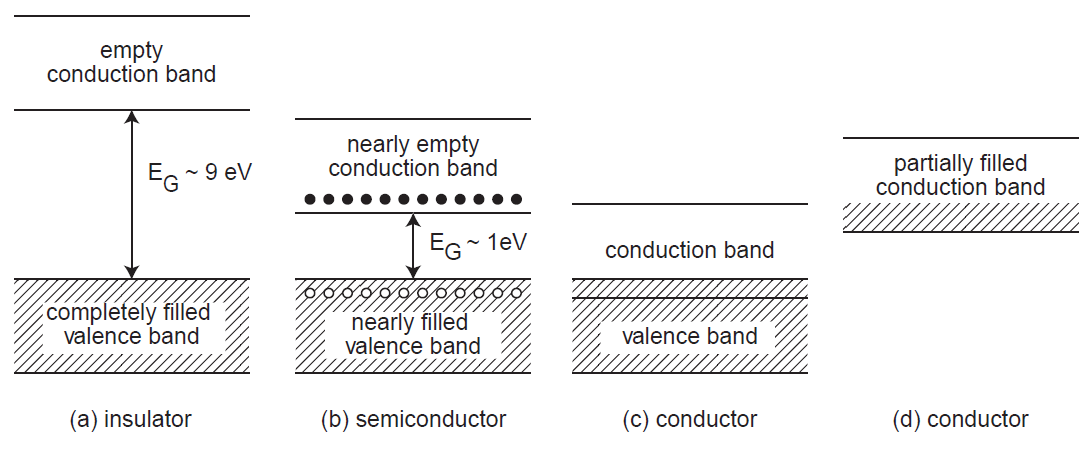
\includegraphics[scale=.6]{energy_band}
\caption{Schematic structure of the energy bands in insulators (a), semiconductors (b) and conductors (c,d).}
\label{fig:energy_band}
\end{figure}


In insulators the valence band electrons are strongly bonded to neighbouring atoms, they are not free and they do not contribute to the conduction. In fact the VB is entirely occupied, the CB instead, is empty. As a consequence of the strong interatomic bond, there are large energy gap between the VB and the CB (typically $E_{G}$ of about 9 GeV). Thus current flow is pratically impossible. 

In semiconductors weaker bonds between neighbouring atoms result in a smaller energy gap with respect to the insulator (for example 1.12 eV in silicon). In this way electrons from VB can easily overcome the gap, moving on the CB by thermal excitations or by external electric fields. When an electron makes this transition, it leaves a hole in the VB, wihch could be filled in turn by another electrons of the VB. If and electric field is applied, the free electrons in the CB and the holes in the VB start to move producing two different current flows, one negative and the other positive, respectively.

In conductors the conduction and valence band overlap or the conduction band is partially filled so transitions within the same band and between the two different bands are easy and current conductions requires minimal energy.


\subsection{Movement of charge carriers and signal formation in semiconductors}

Semiconductor materials are the only ones that allow the detection of charged particles by ionization of the sensitive matter (in conductors a current is always present, not only in case of particle or radiation crossing). 

When a charged particle passes through the medium, it releases a certain amount of energy[, described by the \textit{Bethe-Bloch formula}]. This energy loss, in turn, causes the ionization of the matter and so the formation of positive and negative charges, which in this context, are defined charge carriers. In semiconductors these carrier are the hole electron pairs created by ionization, which  start to move in opposite direction due to an electric field: the holes (positive) migrate towards the \textit{\textbf{anode}} and the electrons (negative) towards the \textit{\textbf{catode}}, which sense the signal induced by this movement. In fact, their drift induce an accumulation of charges on the electrode surfaces, and it is possible to record this charge induction as a charge, current or voltage signal. It is worth to notice that the generation of the signal is dependent on the movement of the carriers relative to the electrodes, and not when they actually arrive, that is the moment in which the signal stop.\\

The charge carrier density of semiconductors can be modified by doping the material with specific chemical elements, and this process causes a modification of their conduction properties.
Undoped semiconductors are called \emph{intrinsic semiconductors}. \\
\emph{Extrinsic semiconductors} instead, are artificially doped with external impurities like: 

\begin{itemize}
\item Pentavalent elements (P, As, Sb), called \emph{donors}, added in a tetravalent material (Si, Ge) produce an axecss of conduction electron with respect to the holes (n doping, \autoref{fig:doping} (a)).
\item Trivalent atoms (B, Al, Ga), called \emph{acceptors}, create an excess of holes (p doping, \autoref{fig:doping} (b)).
\end{itemize}

\begin{figure}[h!]
\centering
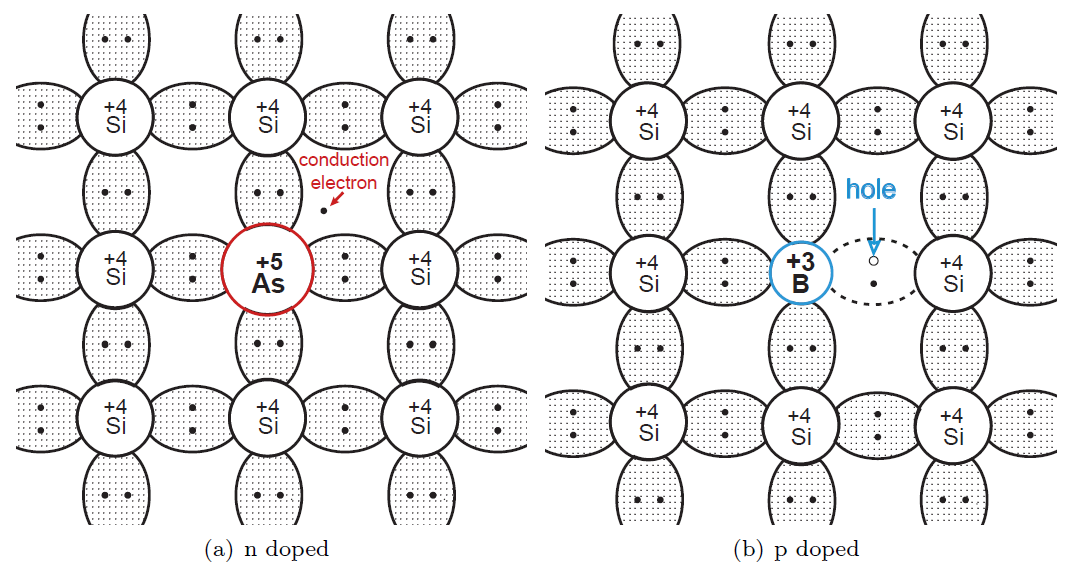
\includegraphics[scale=.6]{doping}
\caption{Schematic representation of atom bonding structure in n-doped and p-doped semiconductors.}
\label{fig:doping}
\end{figure}


%energy necessary to release for silicon
%other semiconductor
%immagine pagina 137, 276, 275, 280 KOLANOSKI


\subsection{The pn junctions as detector}

The base material employed in semiconductor detectors is silicon. When a p-doped semiconductor get in contact with a n-doped material, a \textit{pn junction} is formed. In particular, the p-doped part is the one where holes are the dominant charge carriers, called \textbf{majority carriers}; in the n-doped part of the crystal instead, the majority carriers are the electrons. 
The presence of these excesses of opposite charge in the two part of the junction, causes a migration of the majority carriers from each part to the opposite one. At the boundary the charges recombine, and this process creates a zone which is free of charge carriers, called \textbf{depletion zone}. After the recombination the atoms of this depletion region are ionized and so it is no longer neutral, but features a \emph{space-charge}: a positive one in the n-layer, and a negative in the p-layer. Moreover these space charge densities are opposite in sign, so they generate an intrinsic electrical field that stop the original diffusion.\\

Moreover, the application of an external voltage $V_{ext}$ between the two section of the junction, provokes a variation of the width of the depletion region, depending on the size and polarity of the applied voltage. It is possible to distinguish:

\begin{itemize}
\item \emph{forward bias}, $V_{ext}$>0: a positive external voltage applied to the p side with respect to the n side, causes a reduction of the depletion region ???
\item \emph{reverse bias}, $V_{ext}$<0: if a negative voltage at the p side or positive at the n side relative to the respectively opposite side is applied, the depletion region gets wider.
\end{itemize}

The performance of the junction as a detector is determined above all by the boundary properties between p-and n- doped silicon. Boundaries of the same doping type, but with different concentration, also create a similar pn structure, like for example $n^{+}n$ or $p^{+}p$. There are also Metal-semiconductor boundaries, used in metal contact with the outside and Metal-Oxide-Semiconductor interfaces (MOS) that we will see in more details in the following.
 
\subsection{Complementary Metal-Oxide-Semiconductor (CMOS)}

A MOS structure is a double interface make of three different media: an insulator (oxide) placed between the metal and the semiconductor, as shown in~\autoref{fig:mos}.

\begin{figure}[h!]
\centering
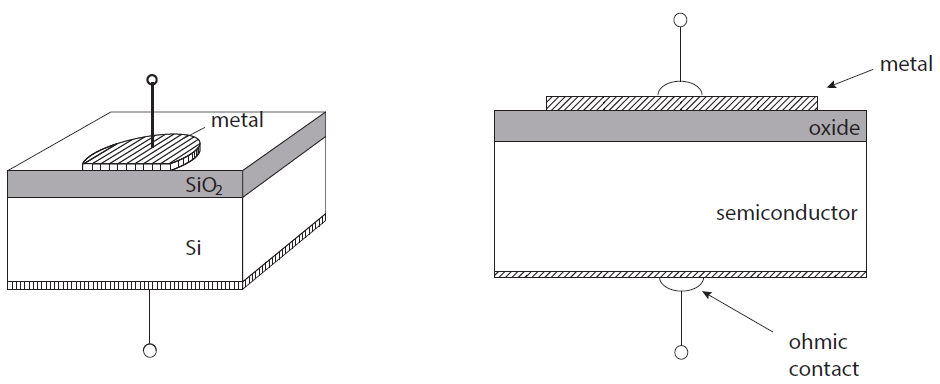
\includegraphics[scale=.6]{mos}
\caption{A perspective (on the left) and a cross-sectional illustration (on the right) of a MOS structure.}
\label{fig:mos}
\end{figure}

In recent transistor technology, the metal is almost entirely replaced by highly doped polysilicon, like $n^{++}$ and $p^{++}$ since these materials are more resistant to high temperature without reacting with the oxide (?). Despite this, the physics remains essentially the same. 
The MOS structure plays a very important role in chip electronics, including the readout of detectors, which employ a combination of NMOS and PMOS transistors, embedded in the substrate. This is st the base of the \emph{Complementary} MOS (CMOS) electronics, which allows to develop more complex circuits. This technique consists in accomodate one of the two transistor type in a differently doped area, called \emph{well}. For example,  in a p-type substrate, a PMOS transistor are accomodate in n-wells, and vice versa with a n-type substrate. 

\section{Hybrid and monolithic pixel sensors}

\subsection{Hybrid}

\subsection{Pixel}


\section{CMOS Monolithic Active Pixel Sensors technology}


\begin{comment}
small fill factor /large fill factor
\end{comment}

\section{History of Monopix developments}

%Articolo Bespin on TJM2




% ARTICOLO 0 (INIZIO TESI)
%CAPITOLO 8 
% MUSTAKAS THESIS
% ARTICOLI VARI
% PRESENTAZIONI
























































%COMMENT


% PRIMA IPOTESI INTRODUZIONE -> SPIEGARE BETHE-BLOCH
\begin{comment}
The detection of elementary particles, nuclei and radiations occurs through their interactions with matter. For example, charge particles are detected by ionization of matter along the trajectory o through the emission of electromagnetic radiation (bremsstrahlung, Cherenkov and transition radiation). Electrons and photons usually develop \textit{electromagnetic showers} in matter. So, all of them interacts by \emph{electromagnetic force}.
Neutrons and other hadrons instead, are revealed employing the \emph{strong interaction} through the formation od \textit{hadronic showers}. Neutrinos, eventually, are detected exploiting the \emph{weak interaction}.

Here we want to sift though the main aspects which characterize the detection of charged particles. 

\subsection{Energy loss by ionization}

The dominant processes which affect the energy loss of charged particles in matter is ionization and excitation of the medium's atoms, at least until the particles reach such high energy that they begin to lose it through radiation.

The average energy loss results from a series of individual stochasti processes, and its behaviour per path lenght is described by the \textit{Bethe-Bloch formula}:

\begin{equation}
-\biggl\langle \frac{dE}{dx} \biggr\rangle = K \frac{Z}{A} \rho \frac{z^{2}}{\beta^{2}} \biggl[ \frac{1}{2} \ln(\frac{2m_{e}c^{2}\beta^{2}\gamma^{2} T_{max}}{I^2}) - \beta^{2} - \frac{\delta(\beta\gamma)}{2} - \frac{C(\beta\gamma,I)}{Z} \biggr]
\label{eq:bethe}
\end{equation}

All the various quantities are explained above:

\begin{itemize}
\item $K = 4\pi N_{A} r^{2} m_{e} c^{2}$ = 0.307 MeV $cm^{2} mol^{-1}$, with the elctron radius $r_{e} = \frac{e^{2}}{4\pi \epsilon_{0} m_{e} c^{2}} \approx 2.8 fm $
\item Z, A, $\rho$ are the atomic number, the atomic mass and the density of the medium, respectively.
\item $z, \beta$ are the charge and the velocity of the particle passing through the matter.
\item I is the mean excitation energy, which describes how easily a target, typically a molecule or atom can absorb kinetic energy from the projectile.
\item $T_{max}$ is the maximum energy that is possible to transfer to a shell electron in a central collision.
\item $\delta$ is the \textit{density correction}, which takes into account a relativistic effect that is the increasing transverse extension of the electric field with $\gamma$.
\item $\frac{C}{Z}$ is a shell correction, relevant for small $\beta$ values.
\end{itemize}

[description of the curve?]

The Bethe-Bloch formula describes the mean energy loss of particles traversing a medium and so it is also called \textit{\textbf{stopping power}}. 
As we mentioned above, the energy loss process has a statistical nature, because it is determined by many ionization or excitation cases, which contributes individually to the formula. Both the number N of total processes and the emitted energy in each one of them, produce fluctuation in the enrgy lost by a particle and as consequence of the energy deposited in the material. They are known as \textit{Landau fluctuations} and they can influence the performance of detectors, so they must be considered. For example in particle identification by the measurement of $\< dE/dx \>$, these fluctuations widen the width of the distribution, worsening the resolution in distinguishing different particle species. In tracking detectors instead, they reduce the space resolution.

[bremss]

\end{comment}


\begin{comment}
There are two type of motions affecting charge carriers moving in electric and magnetic field:

\begin{itemize}
\item An unordered motion with a velocity distribution, classically decribed by the Maxwell-Boltzmann distribution, valid in thermal equilibrium and in absence of an electric field. For example, if there is a concentration gradient in the medium, charges created locally tend to diffuse causing a dispersion of the local charge distribution.
\item A drift movement determined (induced) by the presence of the external electric and magnetic fields. The \textit{drift velocity} $\vec v_{D}$ is the result from a balance between the electric force that aceelerates the charged particles and a friction force arising from collisions with atoms and molecules. In most cases drift velocity is much smaller then the mean velocity $\bigl\langle v \bigr\rangle$.
\end{itemize}


The charge carriers motion in semiconductors is described by the Boltmann transport equation () which includes both diffusion and drift motions (figure). However a specific account on the motion of charge carriers is necessary because lattice phenomena have to be taken into account. 

\begin{description}
\item[DRIFT MOTION]
\end{description}

\begin{description}
\item[DIFFUSION MOTION]
\end{description}

\end{comment}




